\documentclass[tikz,border=10pt]{standalone}
\usepackage{tikz}
\usetikzlibrary{arrows.meta, positioning, calc}

\begin{document}
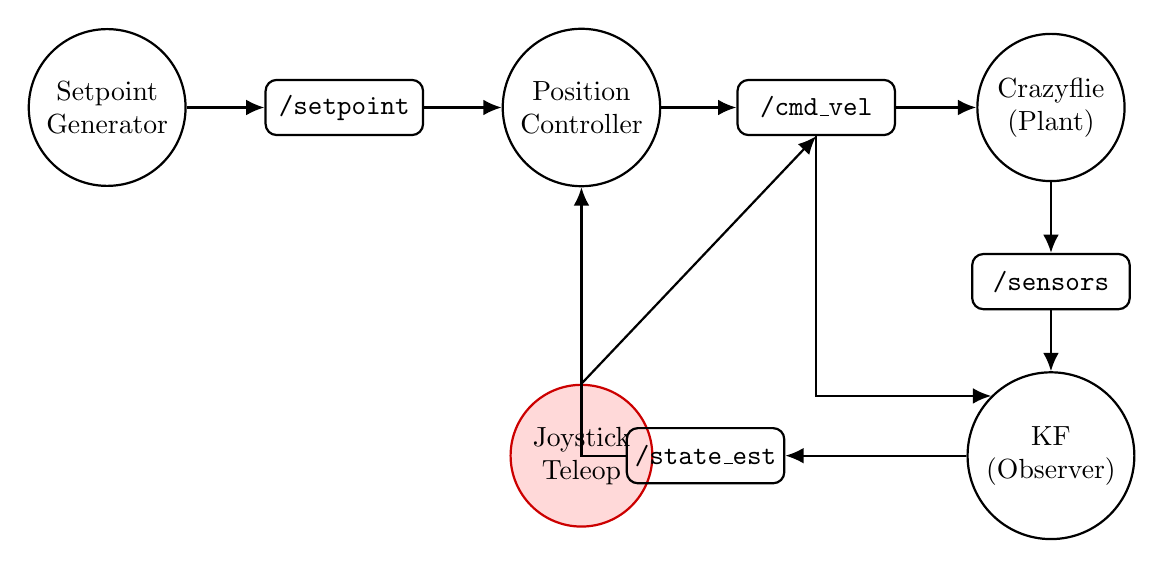
\begin{tikzpicture}[
  node/.style  = {circle, draw, thick, minimum size=18mm, align=center},
  red_node/.style = {circle, draw=red!80!black, fill=red!15, thick, minimum size=18mm, align=center},
  topic/.style = {draw, thick, rounded corners, minimum height=7mm, minimum width=20mm,
                  align=center, inner sep=2pt},
  arrow/.style = {thick, -{Latex[width=2mm]}},
  node distance=3.2cm and 2.2cm
]

%--------------------------------------------------
% ROS nodes (circles)
%--------------------------------------------------
\node[node] (setpoint) {Setpoint\\Generator};
\node[node, right=4.0cm of setpoint] (controller) {Position\\Controller};
\node[node, right=4.0cm of controller] (crazyflie) {Crazyflie\\(Plant)};
\node[node, below=2.4cm of crazyflie] (observer) {KF\\(Observer)};

% Teleop node: south of Controller, same level as observer (RED - external tool)
\node[red_node] (teleop) at (controller |- observer) {Joystick\\Teleop};

%--------------------------------------------------
% Topics (blocks)
%--------------------------------------------------
\node[topic] (t_setpoint) at ($(setpoint)!0.5!(controller)$)
  {\texttt{/setpoint}};

\node[topic] (t_cmd_vel) at ($(controller)!0.5!(crazyflie)$)
  {\texttt{/cmd\_vel}};

\node[topic] (t_sensors) at ($(crazyflie)!0.5!(observer)$)
  {\texttt{/sensors}};

% feedback topic
\node[topic, left=2.3cm of observer.west] (t_state_est)
  {\texttt{/state\_est}};

%--------------------------------------------------
% Connections
%--------------------------------------------------

% Teleop directly to cmd_vel (bypasses setpoint generator and controller)
\draw[arrow] (teleop.north) -- (t_cmd_vel.south);

% setpoint
\draw[arrow] (setpoint.east) -- (t_setpoint.west);
\draw[arrow] (t_setpoint.east) -- (controller.west);

% cmd_vel
\draw[arrow] (controller.east) -- (t_cmd_vel.west);
\draw[arrow] (t_cmd_vel.east) -- (crazyflie.west);

% cmd_vel branch to Observer (south of /cmd_vel -> northwest of Observer)
\draw[arrow]
  (t_cmd_vel.south)
  |- (observer.north west);

% sensors
\draw[arrow] (crazyflie.south) -- (t_sensors.north);
\draw[arrow] (t_sensors.south) -- (observer.north);

% state_est feedback
\draw[arrow] (observer.west) -- (t_state_est.east);
\draw[arrow] (t_state_est.west) -| (controller.south);

\end{tikzpicture}
\end{document}
